\documentclass[10pt]{beamer}
%\documentclass[handout,10pt]{beamer}

\mode<presentation>
{
\usetheme{PI}
}

\usepackage[utf8]{inputenc}
\usepackage[english]{babel}
\usepackage{etex}
\usepackage{listings}
\usepackage{pstricks-add}
\usepackage{url}					
\usepackage{booktabs}			
\usepackage{dcolumn}			
\usepackage{bm}						
\usepackage[left]{eurosym}
\usepackage{subfigure}		
\usepackage{color}				
\usepackage{epstopdf}	
\usepackage[absolute,overlay]{textpos} 
\usepackage{multirow}
\usepackage{textpos}
\usepackage{tikz}
\usepackage{pst-pdf}
\usepackage{graphicx}
\usepackage{pgfpages}

\lstset{
    language=XML,
    keywordstyle=\bfseries\ttfamily\color{blue},
    identifierstyle=\ttfamily\color{black},
    commentstyle=\color[rgb]{0.457,0.723,0.0},
    stringstyle=\ttfamily\color[rgb]{0.627,0.126,0.941},
    showstringspaces=false,
    basicstyle=\scriptsize,
    numberstyle=\scriptsize,
    numbers=left,
    stepnumber=1,
    numbersep=4pt,
    tabsize=2,
    breaklines=true,
    keepspaces=true,
    breakatwhitespace=false,
    aboveskip={1.5\baselineskip},
    columns=flexible,
    frame=single key,
    captionpos=b,
    morekeywords={name,class,threshold,weight,parameter}
    }

%Create Handout?
\only<handout>{\pgfpagesuselayout{4 on 1}[a4paper,landscape]}

%Use BeamerNotes?
%\setbeameroption{show notes on second screen=right}
\graphicspath{{images/}}

\title[SiLift]{High-level Differencing, Patching and Merging of EMF Models}
%\subtitle{SubTitle}
\author[D. Reuling \\ M. Ohrndorf]{Dennis Reuling -- Manuel Ohrndorf}
\date[18.11.2013]{Eclipse DemoCamp}
\pgfdeclareimage[height=1.5cm]{titlegraphic}{logoTitle}
\titlegraphic{\pgfuseimage{titlegraphic}}

\hypersetup{
	pdfauthor={Dennis Reuling, Manuel Ohrndorf},
    pdfsubject={SiLift: High-level Differencing, Patching and Merging of EMF Model}
	pdfkeywords={SiLift, EMF Compare, Differences, Operations, Lifting, Patching,
	Merging} }

%\beamerdefaultoverlayspecification{<+$\rightarrow$}

\begin{document}

 \pgfdeclareverticalshading{fadeBlue}{\paperwidth}%
 {color(0cm)=(bg);color(1cm)=(structure.fg!25!structure.bg)}

\begingroup
\makeatletter
%\setbeamertemplate{background canvas}[vertical shading][top=bg,bottom=structure.fg!25!structure.bg]
\only<presentation>{\setlength{\hoffset}{-25pt}}
\beamertemplatenavigationsymbolsempty
\makeatother
\begin{frame}[plain]
    \titlepage
\end{frame}
\endgroup

%no subsections in toc
\setcounter{tocdepth}{1}

\begingroup
\makeatletter
\setbeamertemplate{sidebar left}{}
\makeatother
\begin{frame}
\frametitle{About us}
\begin{block}{Software Engineering Group, University of Siegen}
Main research area: Model driven software development \\
\medskip
\textbf{Web:} \url{http://pi.informatik.uni-siegen.de}
\end{block}
\begin{block}{Dennis Reuling, M. Sc.}
Research Scientist at SEG\\
%\medskip
%\textbf{Thesis:} Integration of UML Profiles into the SiDiff and SiLift tools
% based on a SysML case study \\
\medskip
\textbf{Email:} \url{dreuling@informatik.uni-siegen.de}

\end{block}
\begin{block}{Manuel Ohrndorf, B. Sc.}
Research Assistant at SEG \\
%\medskip
%\textbf{Thesis:} Generation of transformation rules for the optimization of
% model differences\\
\medskip
\textbf{Email:} \url{mohrndorf@informatik.uni-siegen.de}
\end{block}
\end{frame}
\endgroup

\begingroup
\makeatletter
\setbeamertemplate{sidebar left}{}
\makeatother
\begin{frame}
  \frametitle{Agenda}
  \tableofcontents
\end{frame}
\endgroup

\AtBeginSection[]%
{%
\frame{\sectionpage}
}

\section{Introduction}
\begin{frame}
\frametitle{Use Cases of SiLift}
\begin{columns}[t]
\begin{column}{0.5\textwidth}
\begin{block}{Differencing}
  \begin{center}
\includegraphics[scale=0.47]{images/createPatch}
  \end{center}
\end{block}
\end{column}
\begin{column}{0.5\textwidth}
\begin{block}{Patching}
  \begin{center}
\includegraphics[scale=0.41]{images/applyPatch}
  \end{center}
\end{block}
\end{column}
 \end{columns}

\begin{block}{Merging}
  \begin{center}
\includegraphics[scale=0.55]{images/applyPatchMerge}
  \end{center}
\end{block}
\end{frame}
\begin{frame}[t]
  \frametitle{Model Evolution}
  \begin{flushleft}
  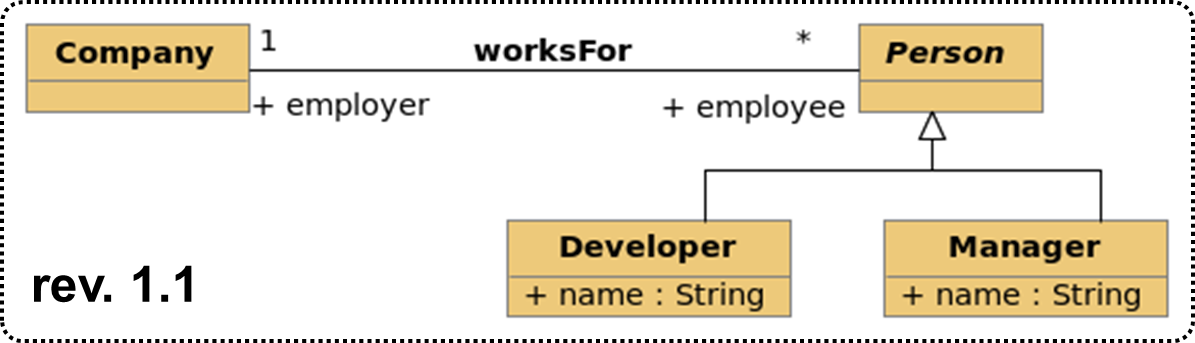
\includegraphics[scale=0.46]{images/uml_example_01}
  \end{flushleft}
\end{frame}

\begin{frame}[t,noframenumbering]
  \frametitle{Model Evolution}
  \begin{flushleft}
  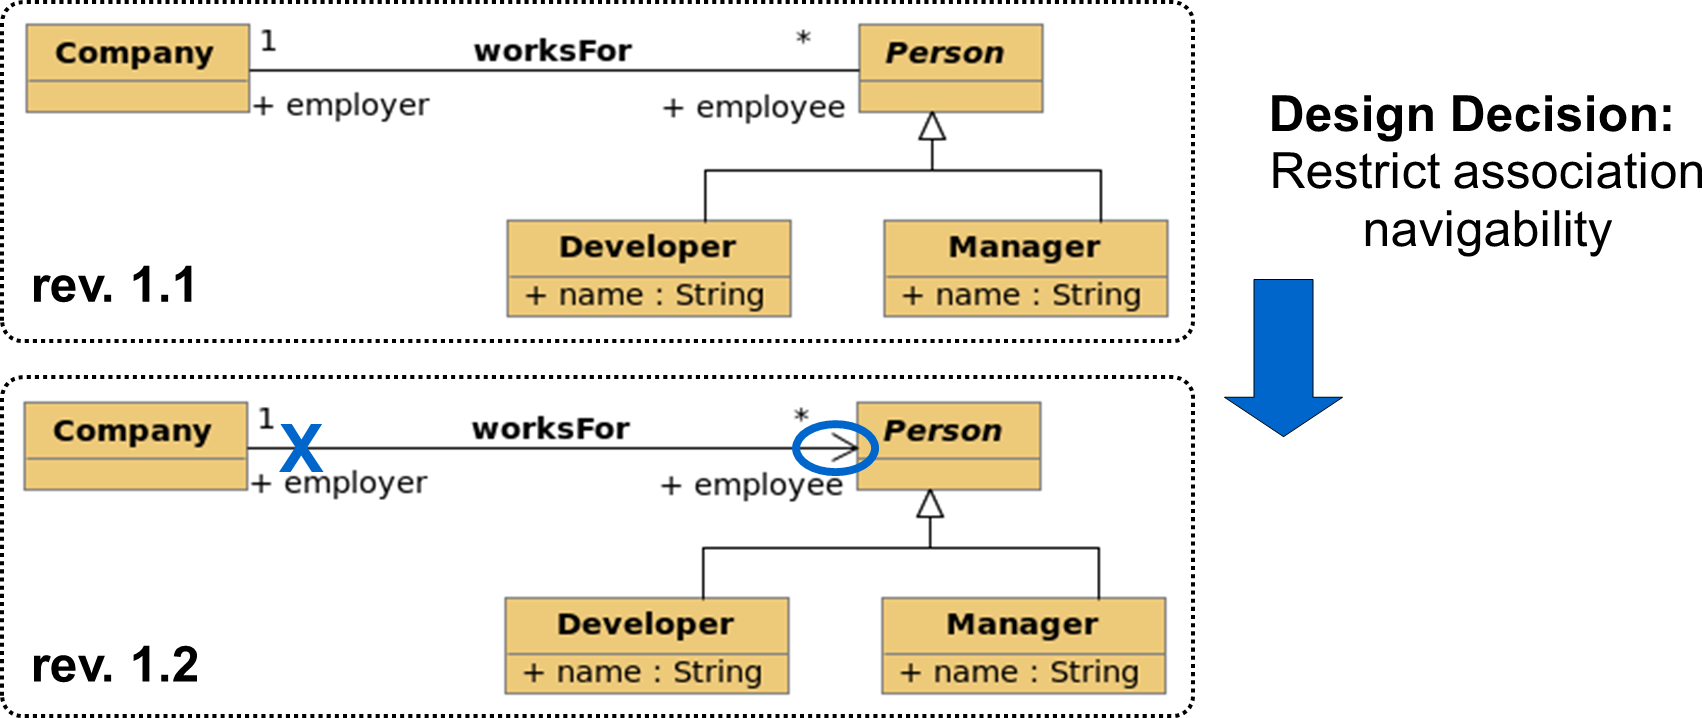
\includegraphics[scale=0.46]{images/uml_example_02}
  \end{flushleft}
\end{frame}

\begin{frame}[t,noframenumbering]
  \frametitle{Model Evolution}
  \begin{flushleft}
  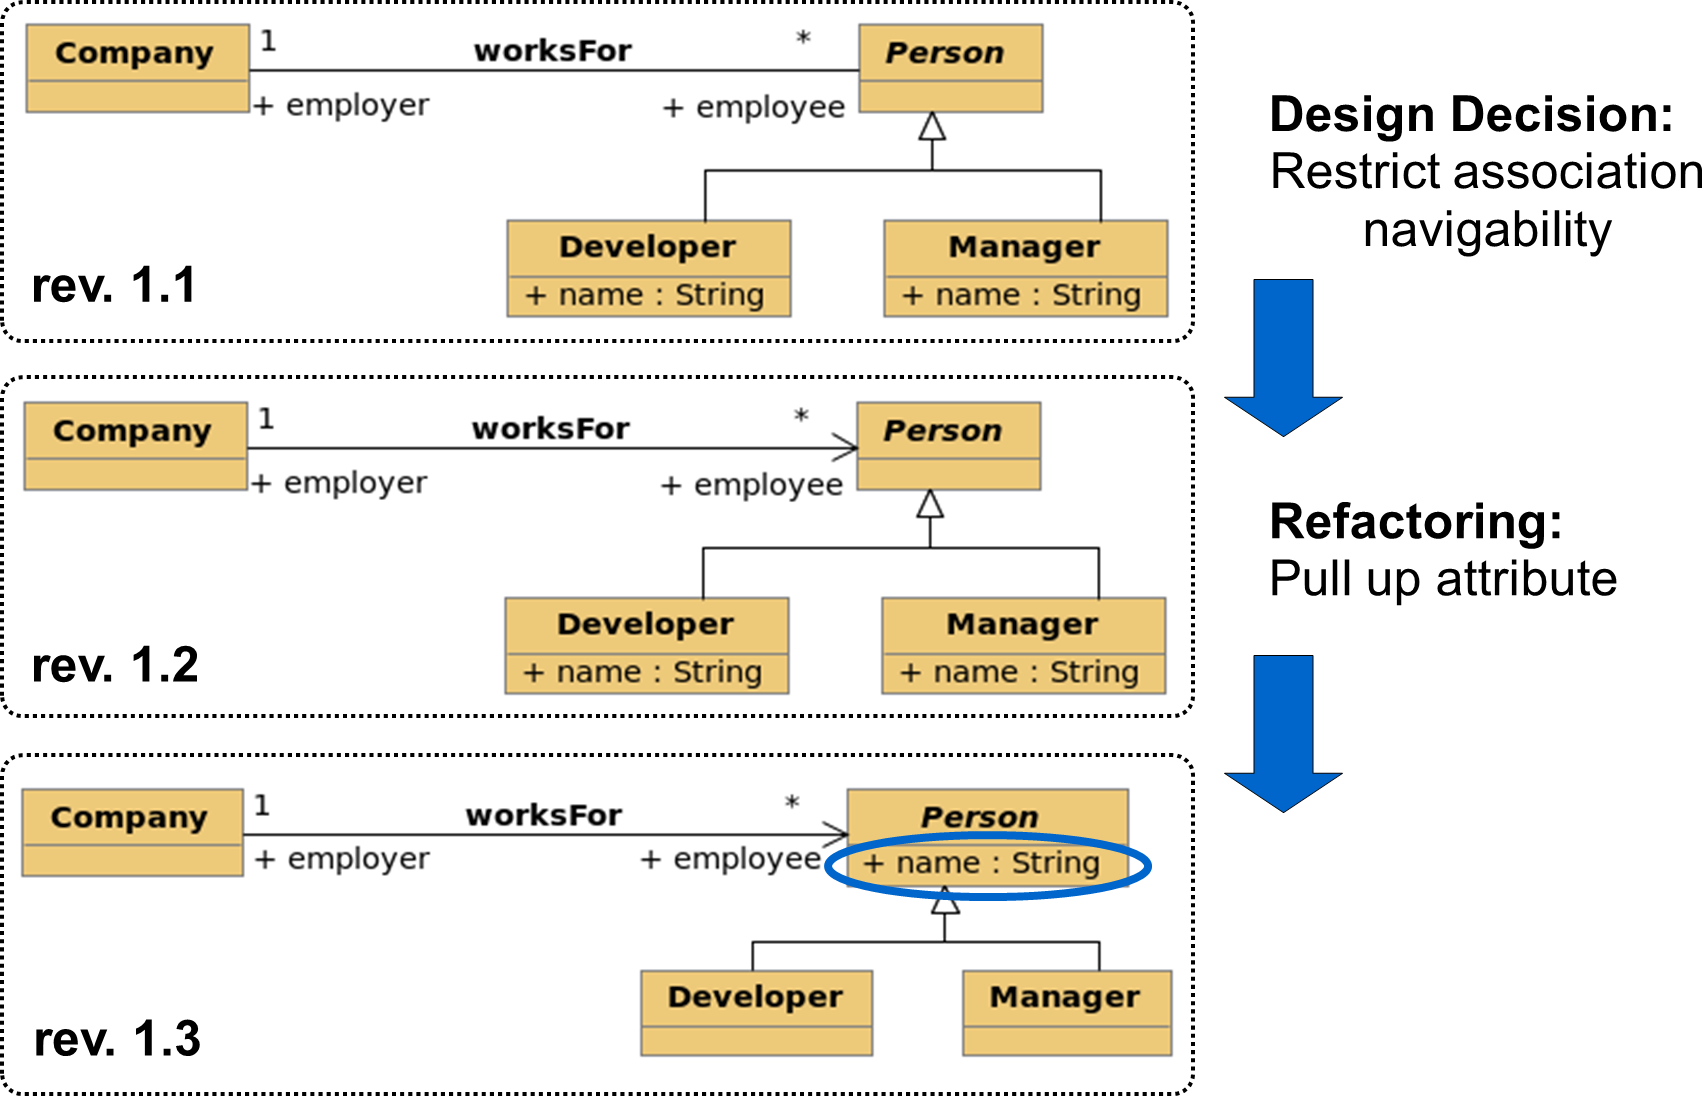
\includegraphics[scale=0.46]{images/uml_example_03}
  \end{flushleft}
\end{frame}

\begin{frame}
  \frametitle{Model Evolution}
  \begin{center}
  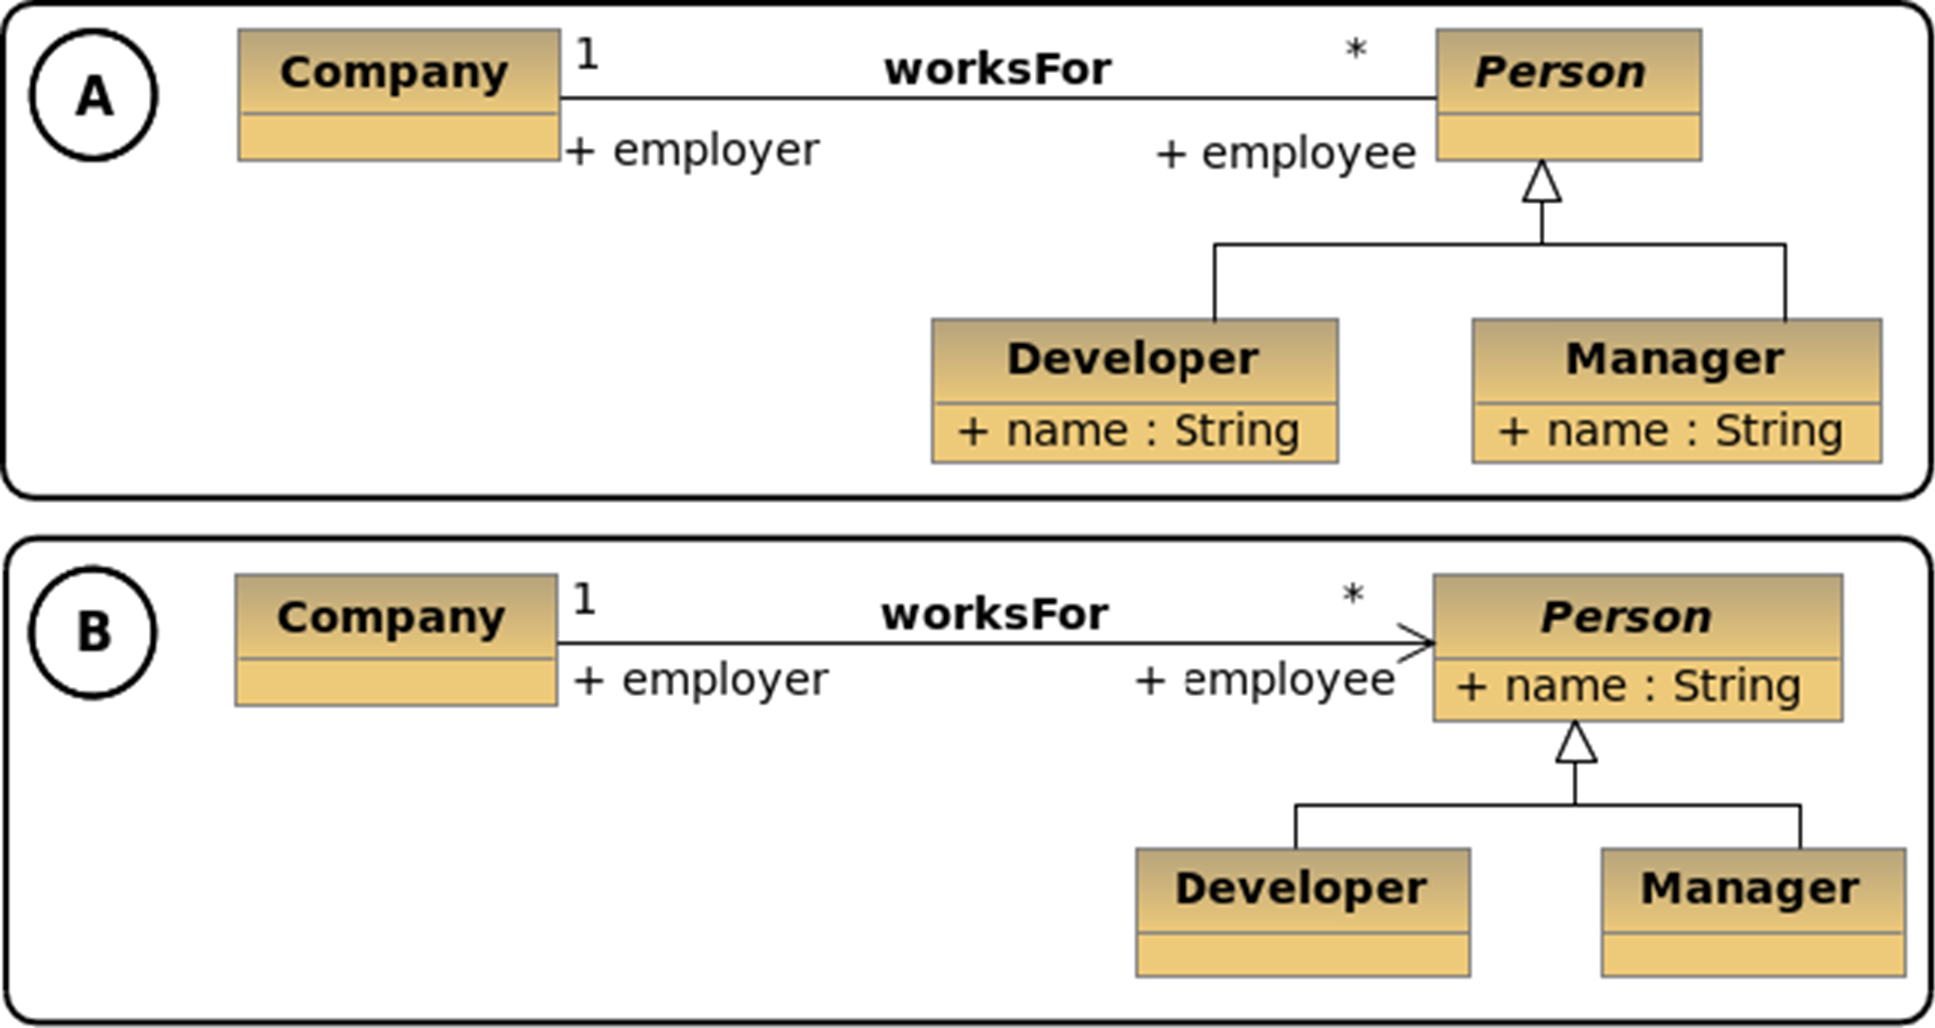
\includegraphics[scale=0.4]{images/uml_example_04}
  \end{center}
\end{frame}

\begin{frame}
  \frametitle{What textual difference tools report\ldots}
  \begin{center}
  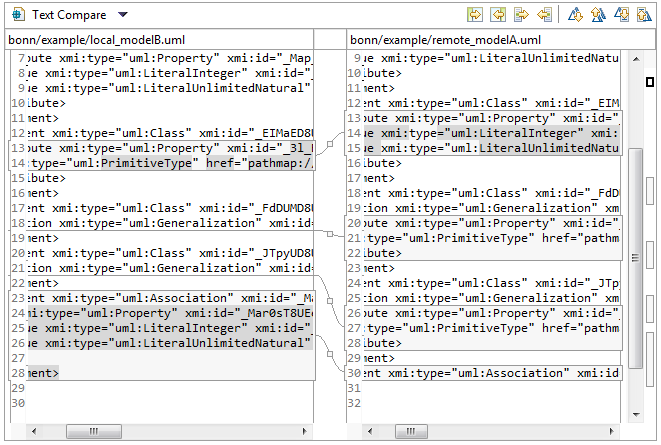
\includegraphics[scale=0.55]{images/text_compare}
  \end{center}
\end{frame}

\begin{frame}
  \frametitle{What EMFCompare reports\ldots}
  \begin{center}
  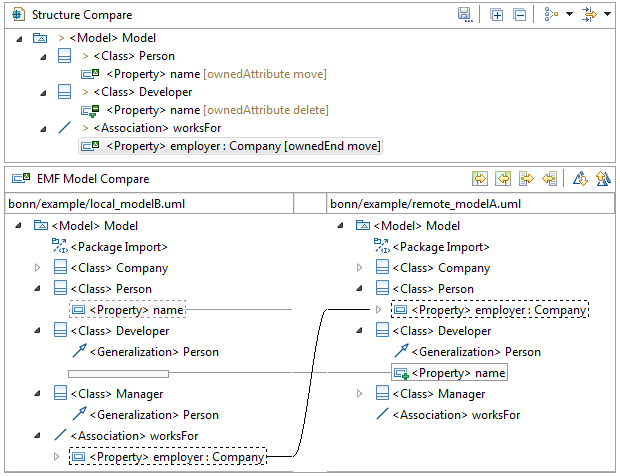
\includegraphics[scale=0.55]{images/emf_compare}
  \end{center}
\end{frame}
\begin{frame}[t]
  \frametitle{Model Evolution}
  \begin{flushleft}
  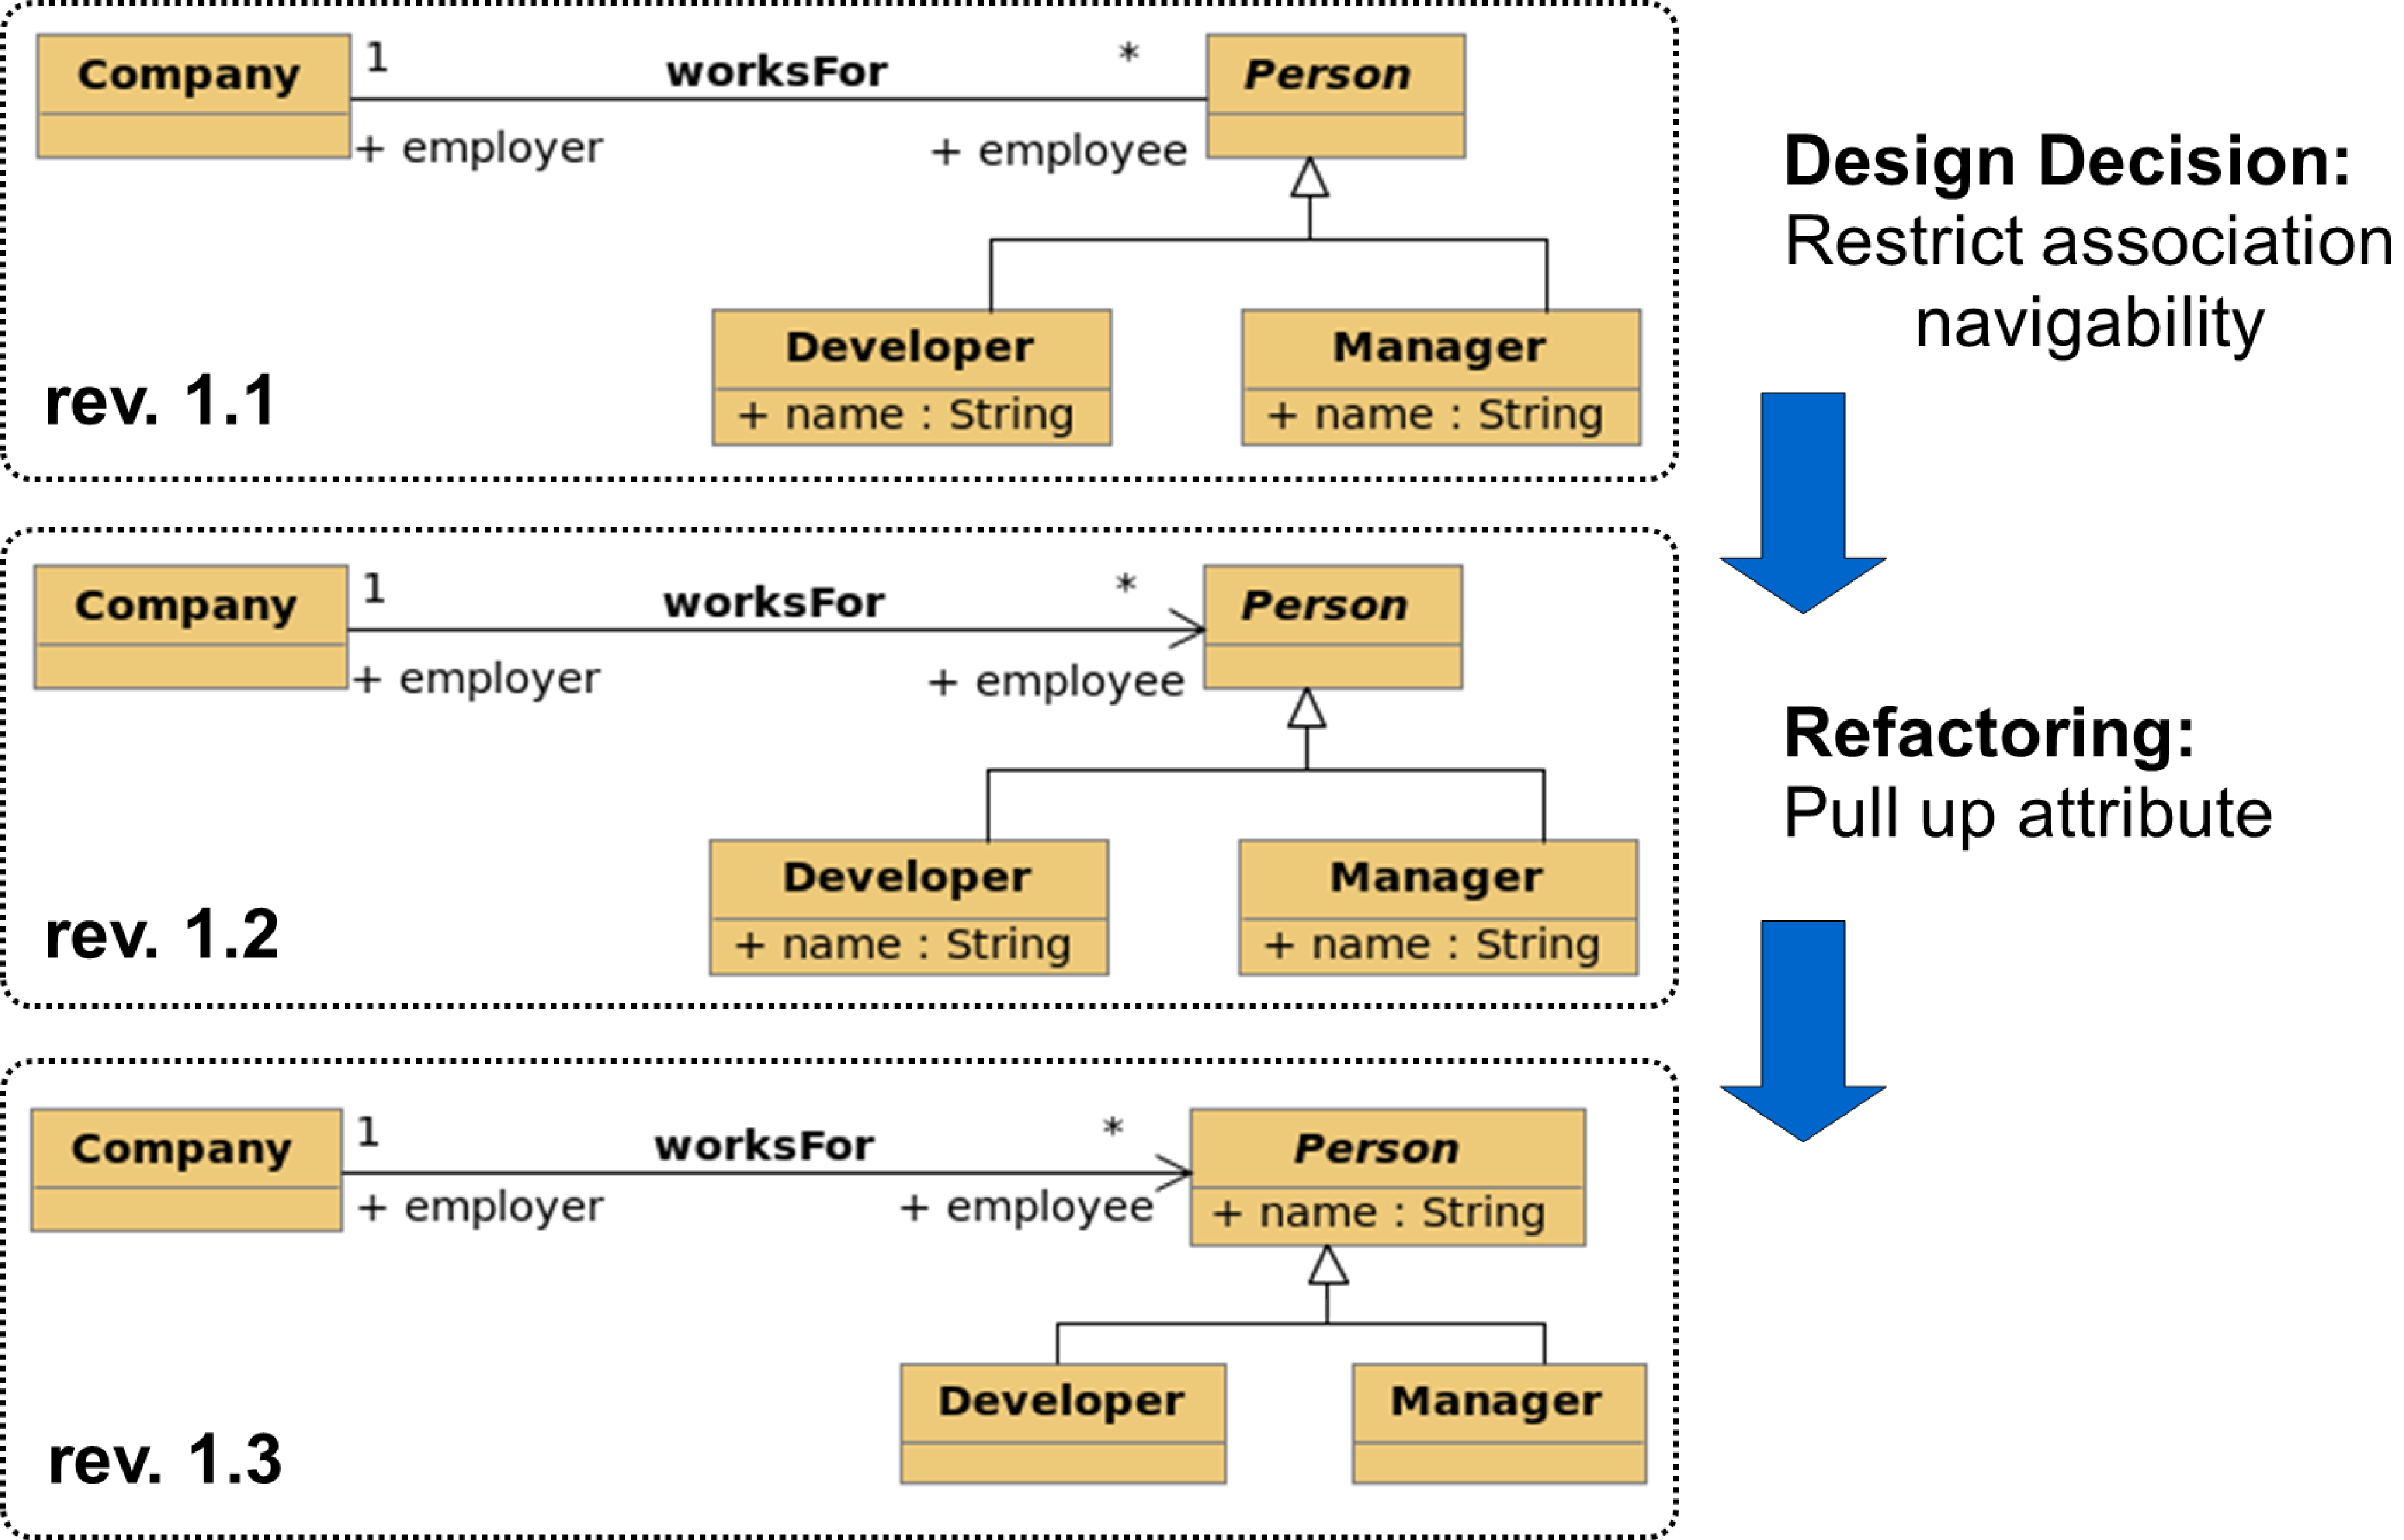
\includegraphics[scale=0.2]{images/uml_example_05_01}
  \end{flushleft}
\end{frame}
\begin{frame}[t,noframenumbering]
  \frametitle{Model Evolution}
  \begin{flushleft}
  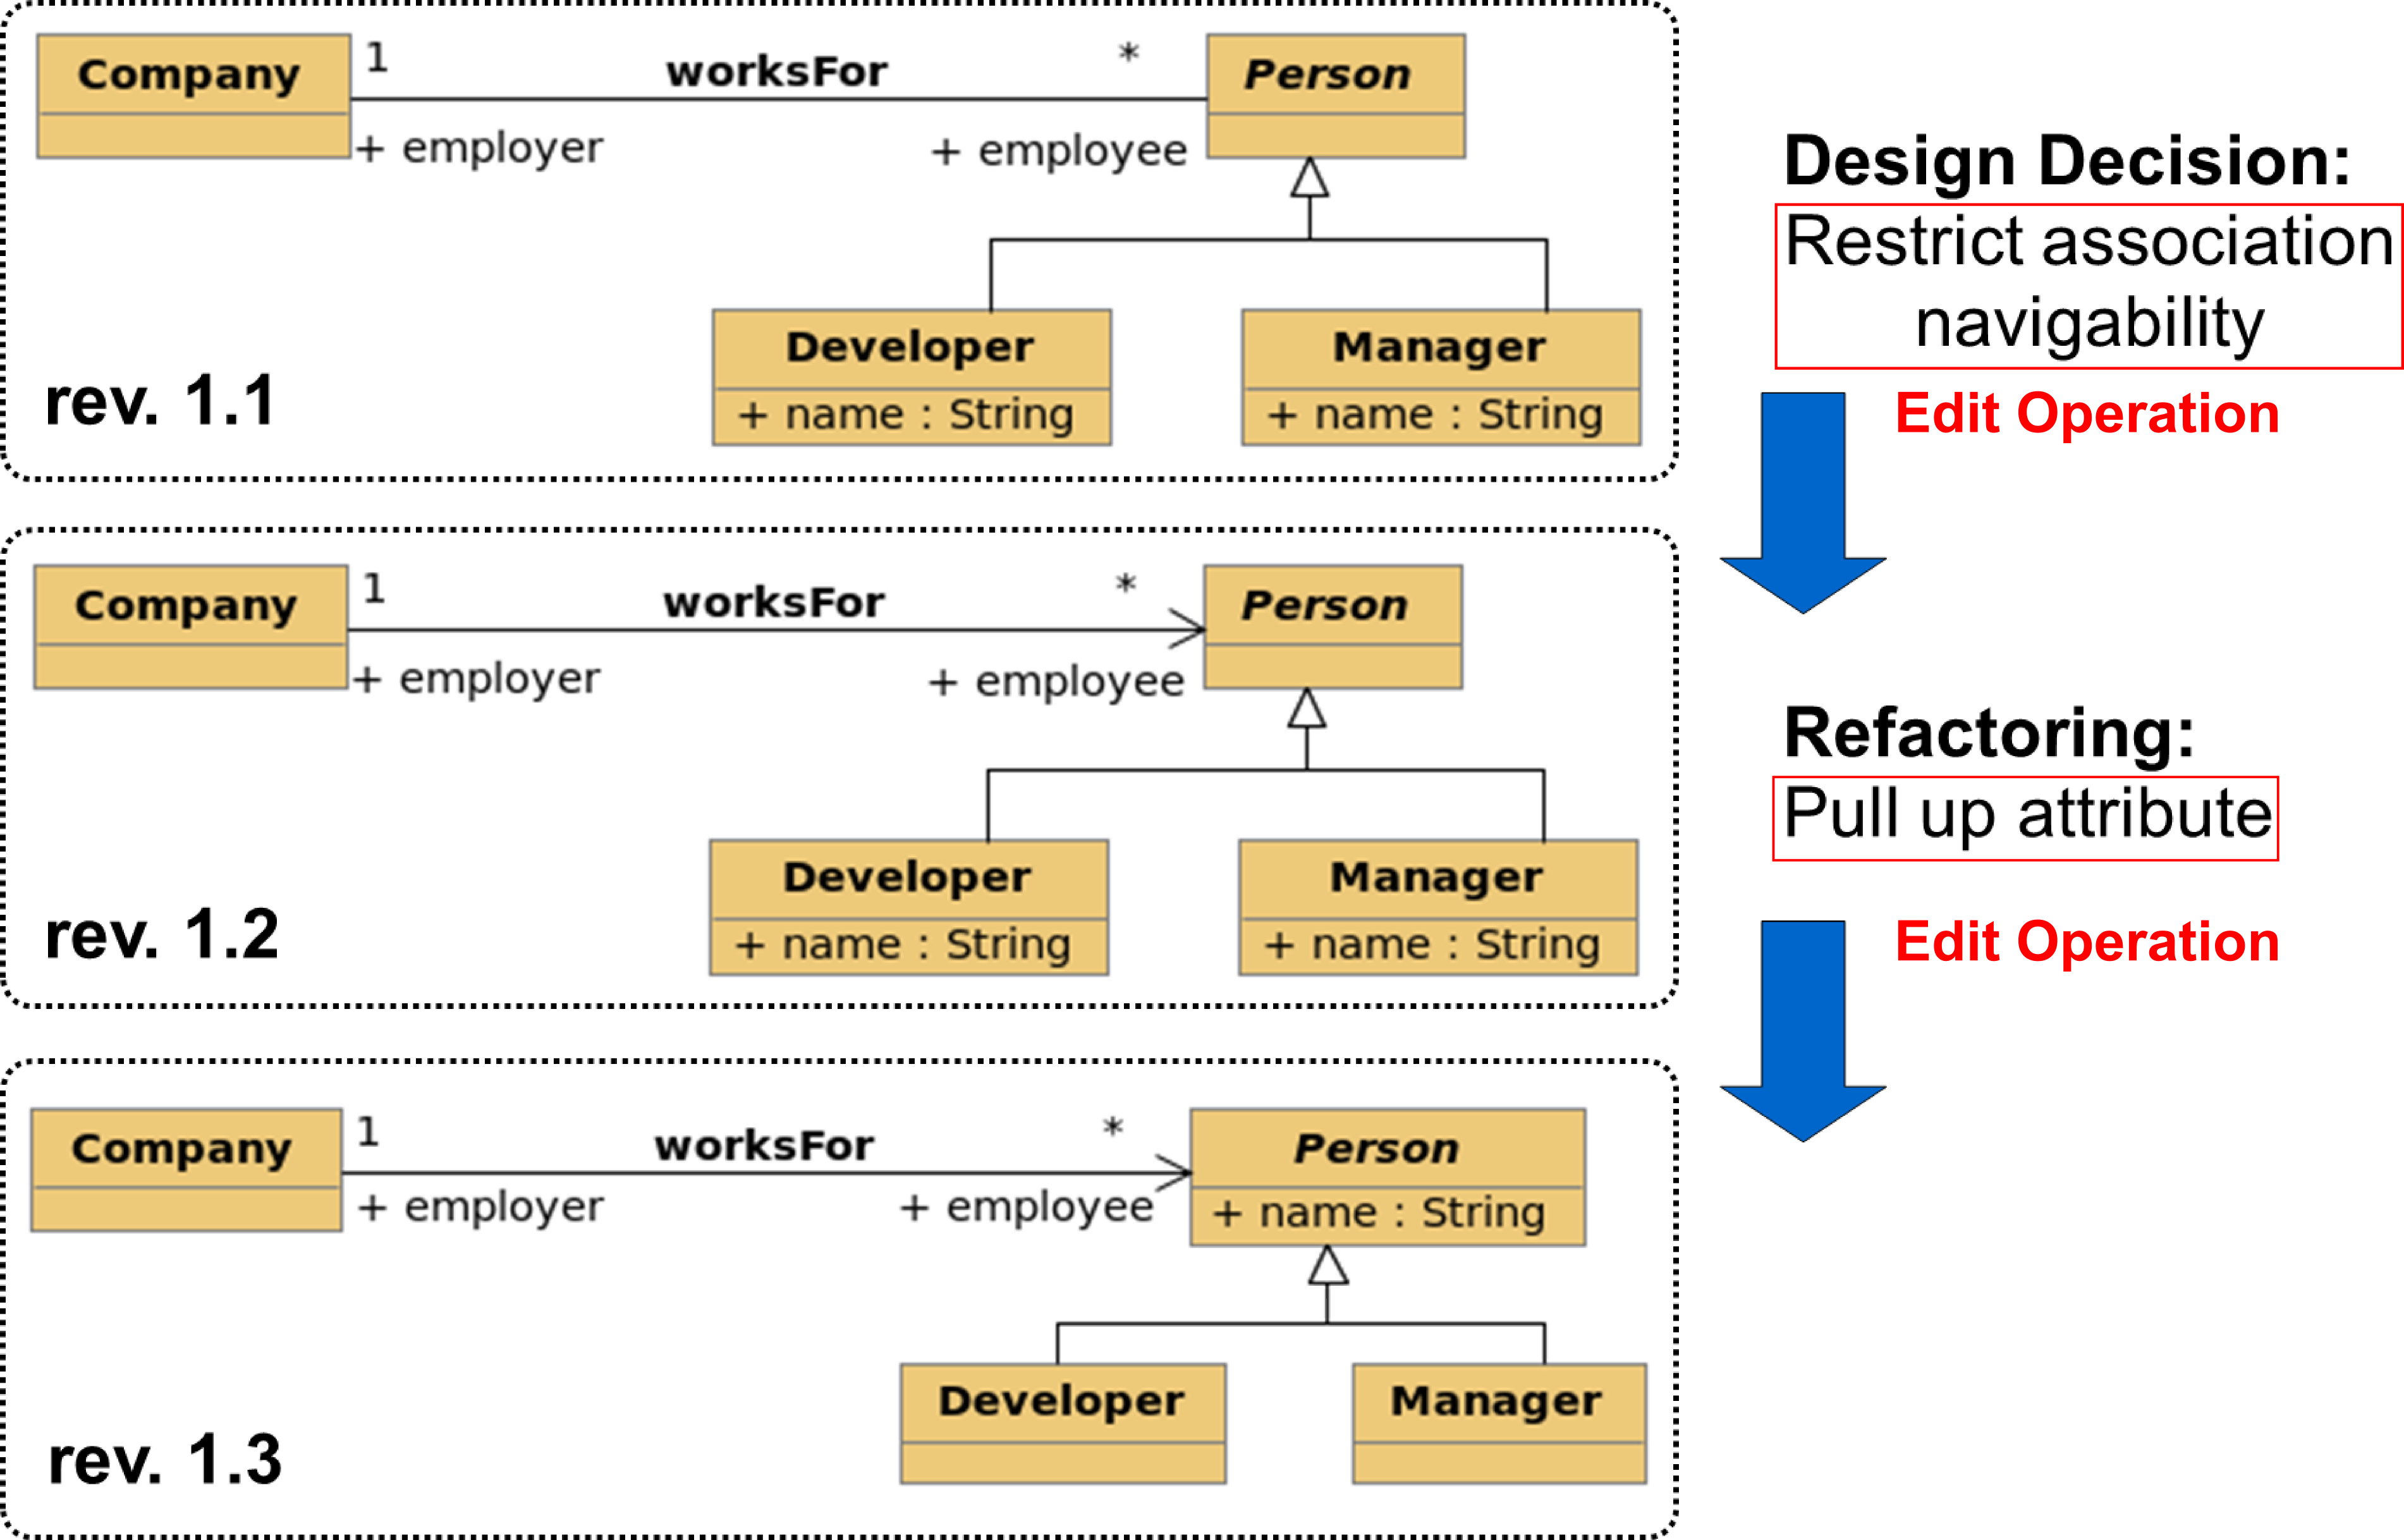
\includegraphics[scale=0.2]{images/uml_example_05_02}
  \end{flushleft}
\end{frame}
% \begin{frame}
%   \frametitle{What SiLift reports\ldots}
%   \begin{center}
%   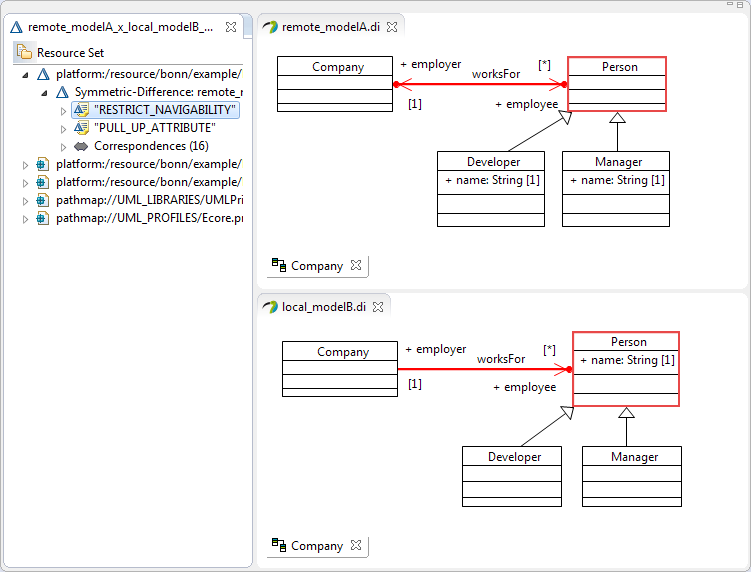
\includegraphics[scale=0.5]{images/symmetric_collapsed}
%   \end{center}
% \end{frame}
\section{SiLift Tools}
\begin{frame}
\frametitle{Use Case (1)}
\begin{block}{Differencing}
  \begin{center}
\includegraphics[scale=0.5]{images/createPatch}
  \end{center}
\end{block}
\end{frame}
\begin{frame}
  \frametitle{Difference Viewer}
  \begin{center}
 % \includegraphics[scale=0.4]{images/createPatch} \\ 
 % \medskip
  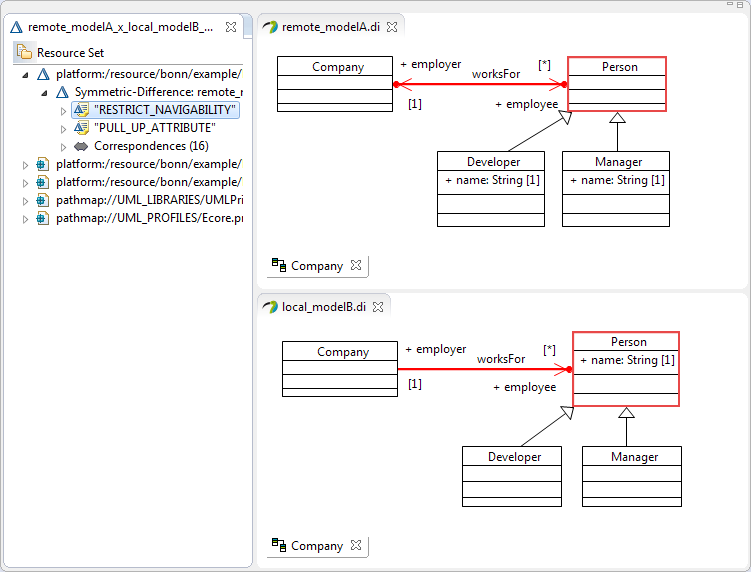
\includegraphics[scale=0.5]{images/symmetric_collapsed}
  \end{center}
\end{frame}
\begin{frame}
\frametitle{Use Case (2)}
\begin{block}{Patching}
  \begin{center}
\includegraphics[scale=0.5]{images/applyPatch}
  \end{center}
\end{block}
\end{frame}
\begin{frame}
  \frametitle{Consistency-Preserving Editing of Patches (1)}
  \begin{center}
 % 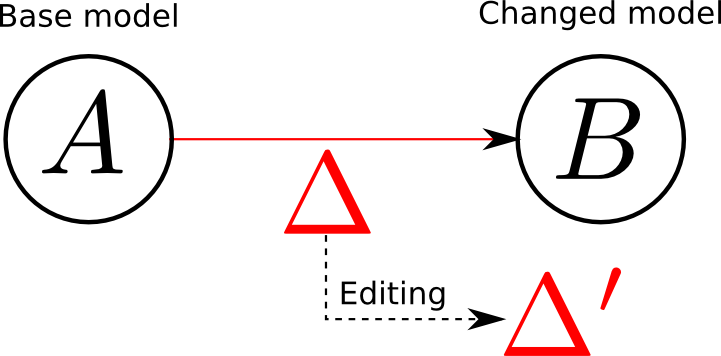
\includegraphics[scale=0.4]{images/editPatch} \\ 
 % \medskip
  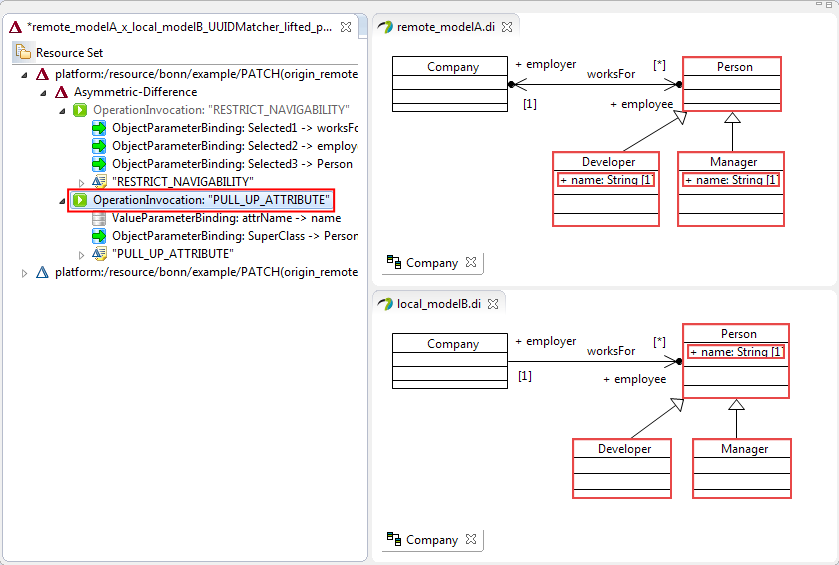
\includegraphics[scale=0.425]{images/asymmetric_pull_up_attribute_1}
  \end{center}
\end{frame}
\begin{frame}[noframenumbering]
  \frametitle{Consistency-Preserving Editing of Patches (2)}
  \begin{center}
 % 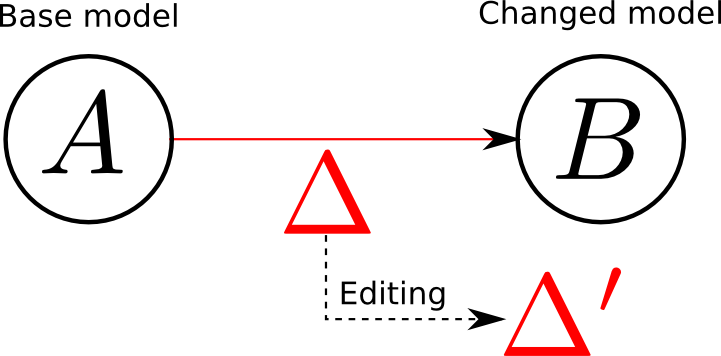
\includegraphics[scale=0.4]{images/editPatch} \\ 
 % \medskip
  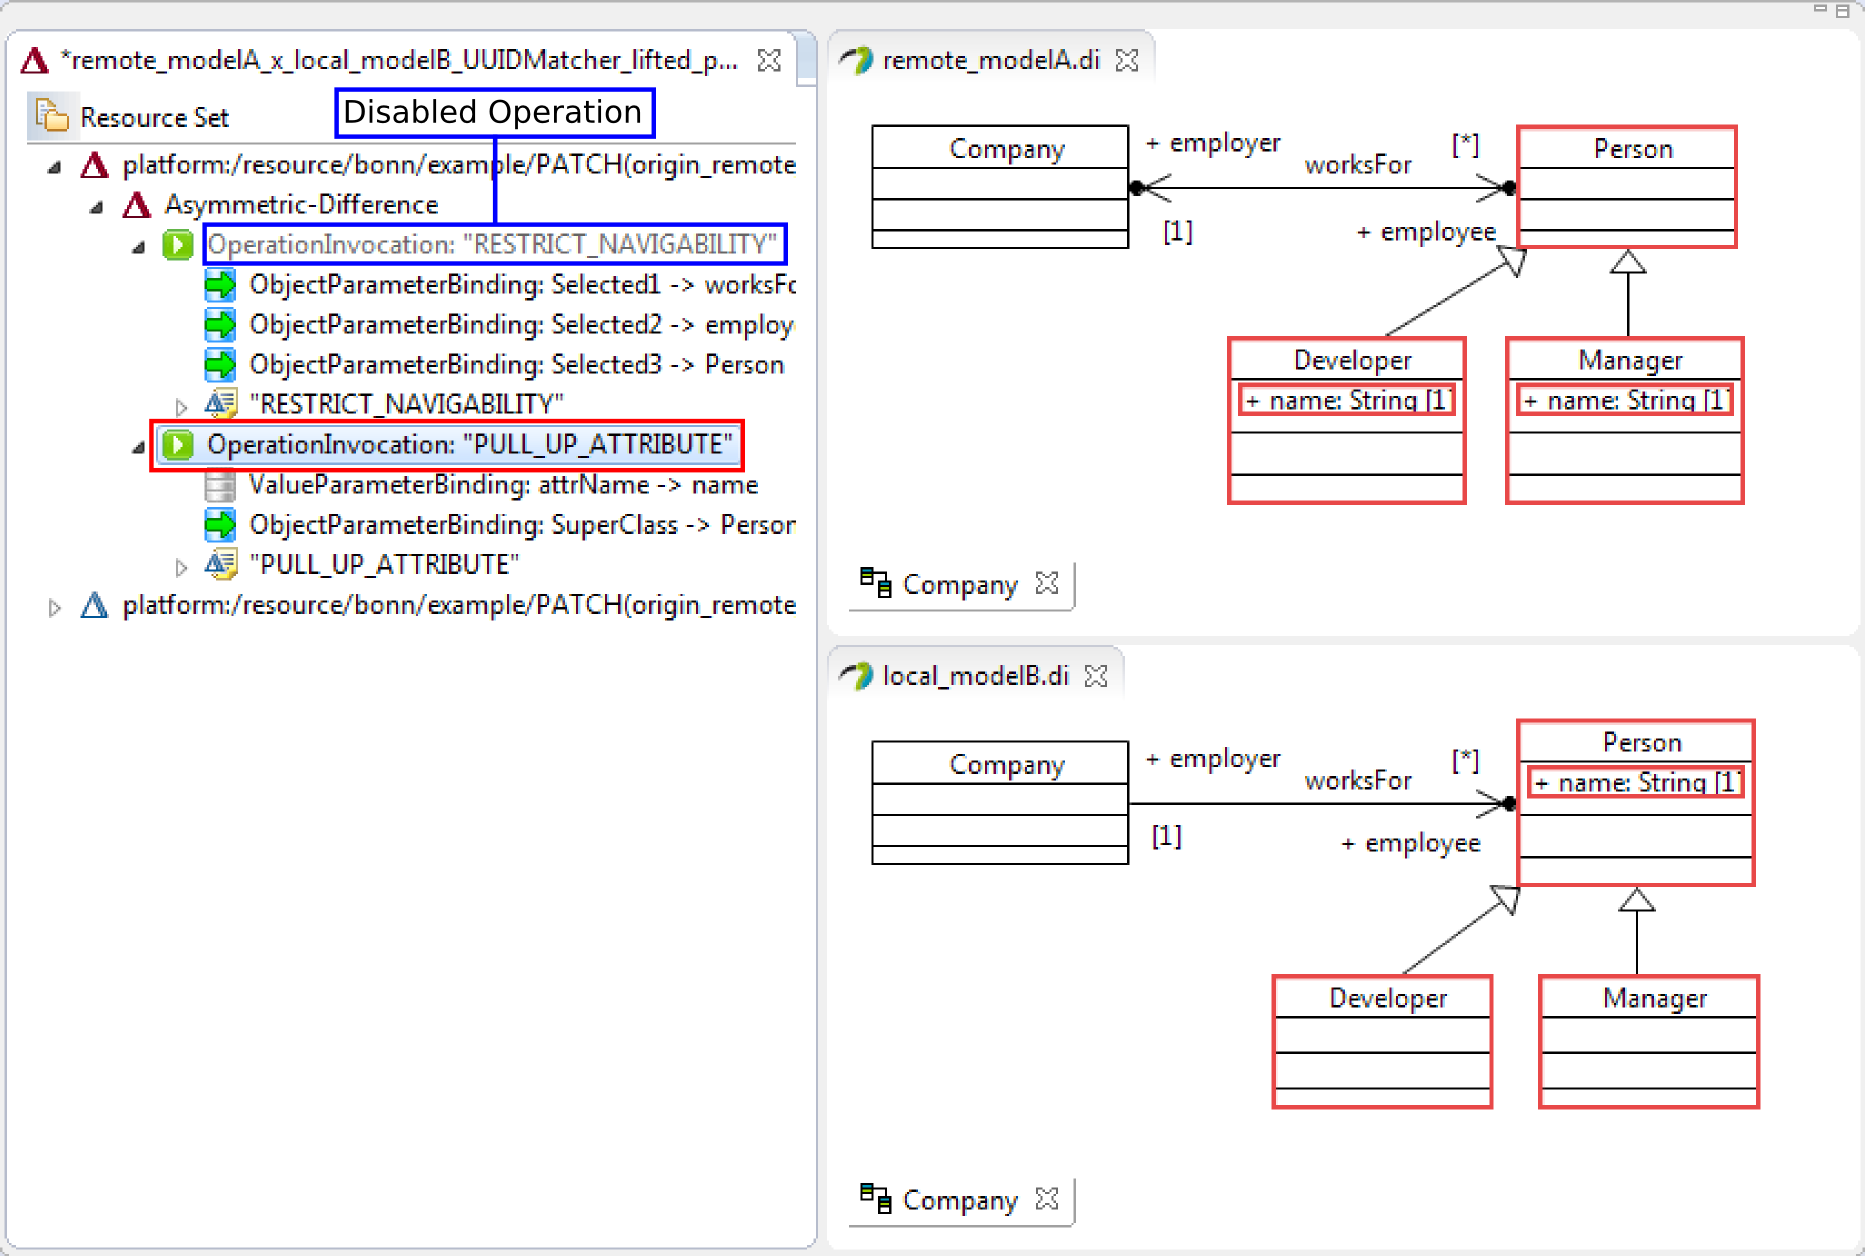
\includegraphics[scale=0.425]{images/asymmetric_pull_up_attribute_2}
  \end{center}
\end{frame}
\begin{frame}
  \frametitle{Controlled Application of Model Patches (1)}
  \begin{center}
 % \includegraphics[scale=0.4]{images/applyPatch} \\ 
 % \medskip
  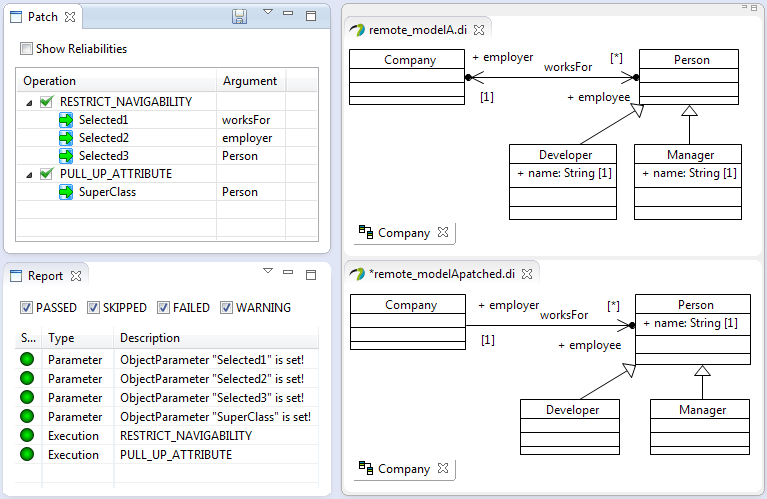
\includegraphics[scale=0.45]{images/patch_01_1}
  \end{center}
\end{frame}
\begin{frame}[noframenumbering]
  \frametitle{Controlled Application of Model Patches (2)}
  \begin{center}
 % \includegraphics[scale=0.4]{images/applyPatch} \\ 
 % \medskip
  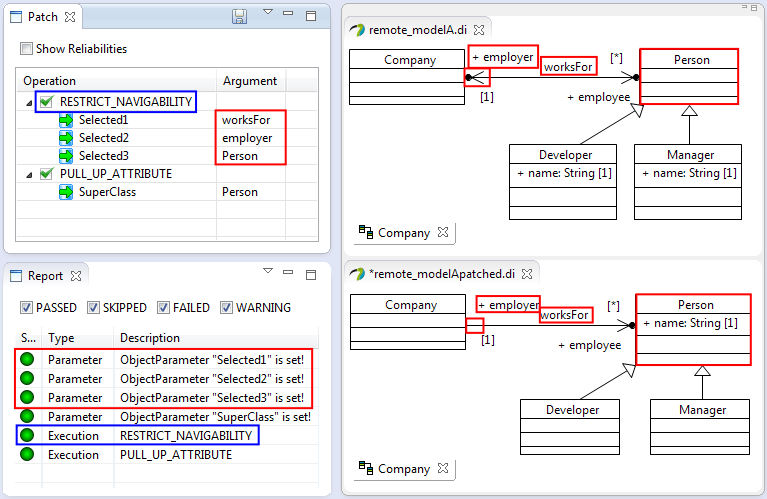
\includegraphics[scale=0.45]{images/patch_01_2}
  \end{center}
\end{frame}
\begin{frame}[noframenumbering]
  \frametitle{Controlled Application of Model Patches (3)}
  \begin{center}
 % \includegraphics[scale=0.4]{images/applyPatch} \\ 
 % \medskip
  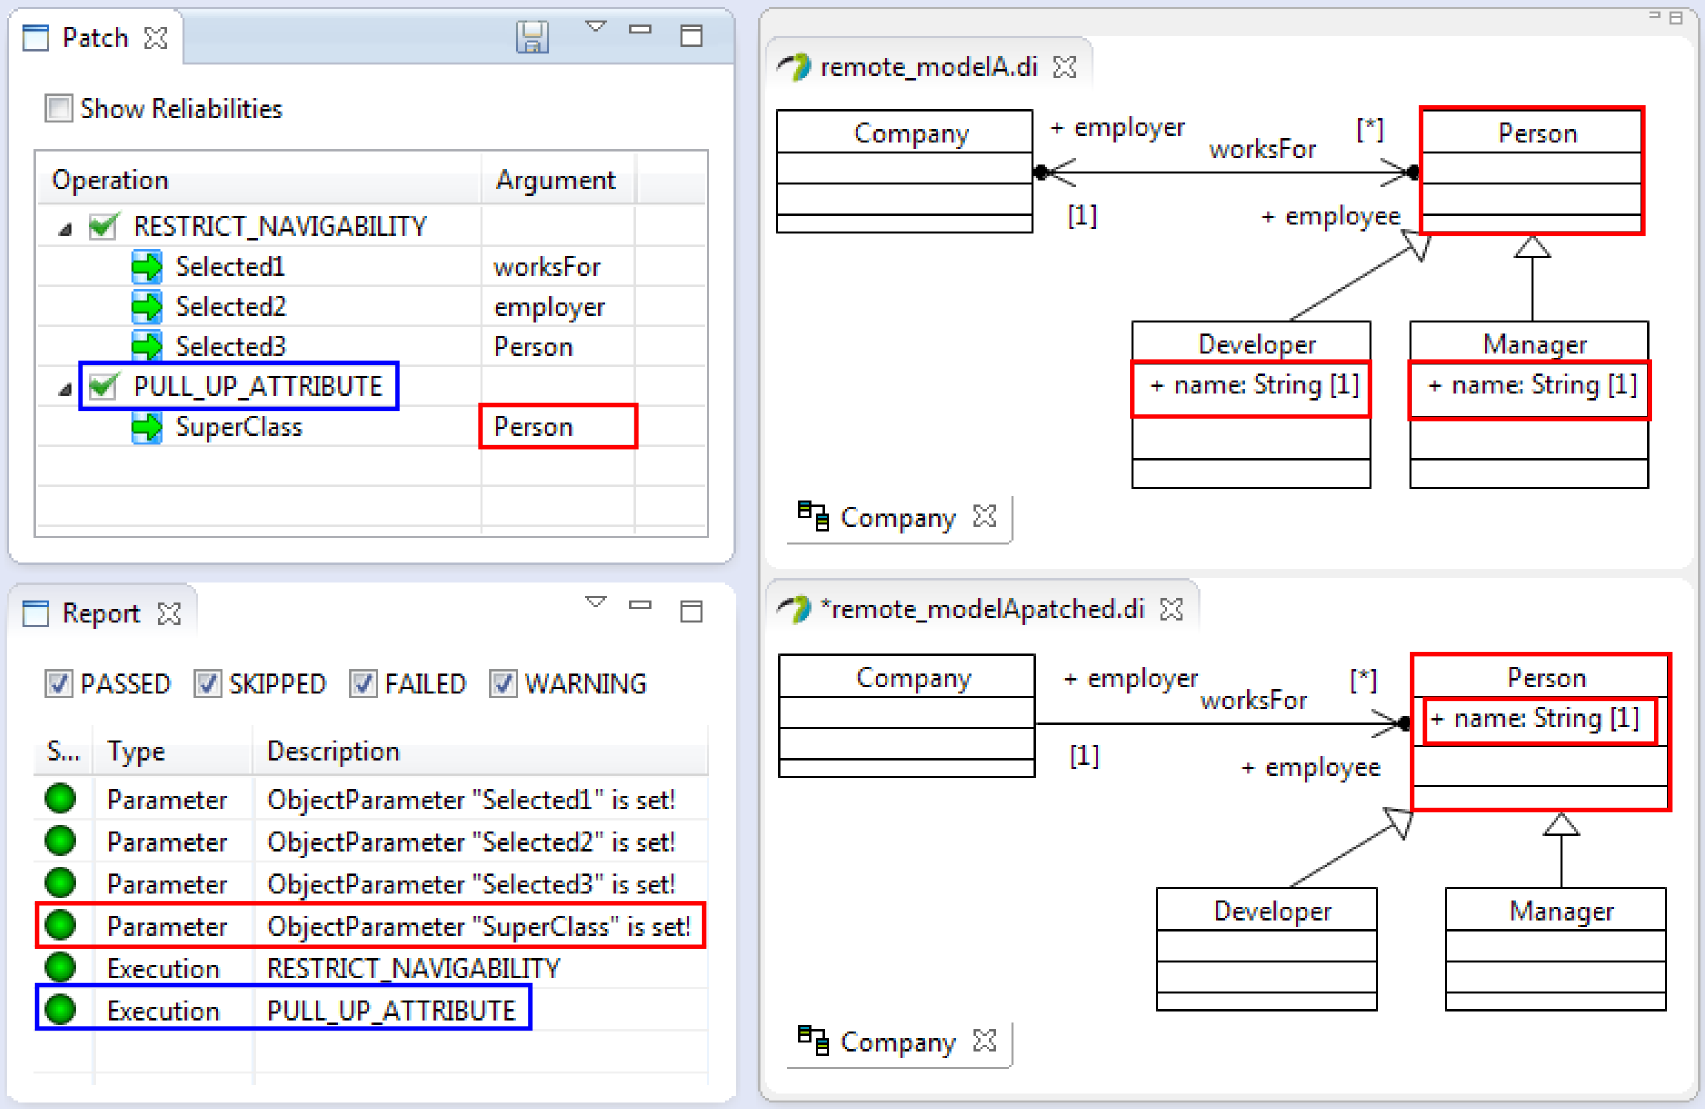
\includegraphics[scale=0.45]{images/patch_01_3}
  \end{center}
\end{frame}
\begin{frame}
\frametitle{Use Case (3)}
\begin{block}{Merging}
  \begin{center}
\includegraphics[scale=0.5]{images/applyPatchMerge}
  \end{center}
\end{block}
\end{frame}
\begin{frame}
  \frametitle{Controlled Merging (1)}
  \begin{center}
 % \includegraphics[scale=0.4]{images/applyPatchMerge} \\ 
 % \medskip
  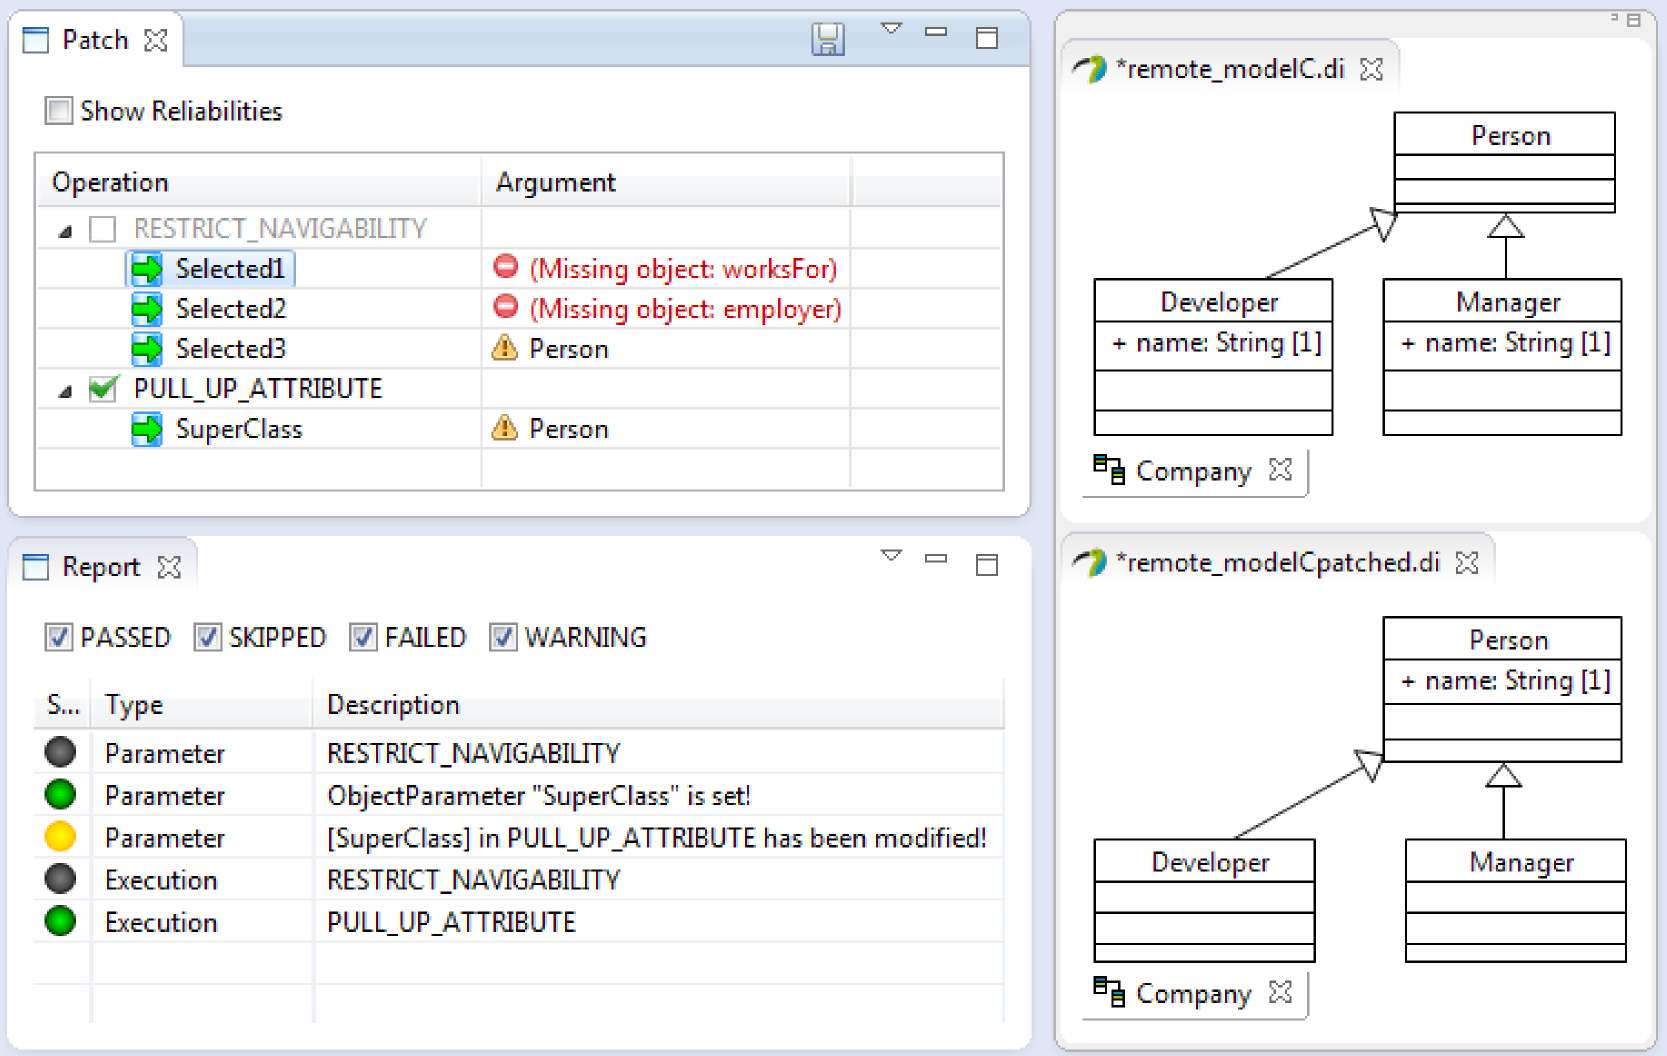
\includegraphics[scale=0.45]{images/patch_02_1}
  \end{center}
\end{frame}
\begin{frame}[noframenumbering]
  \frametitle{Controlled Merging (2)}
  \begin{center}
 % \includegraphics[scale=0.4]{images/applyPatchMerge} \\ 
 % \medskip
  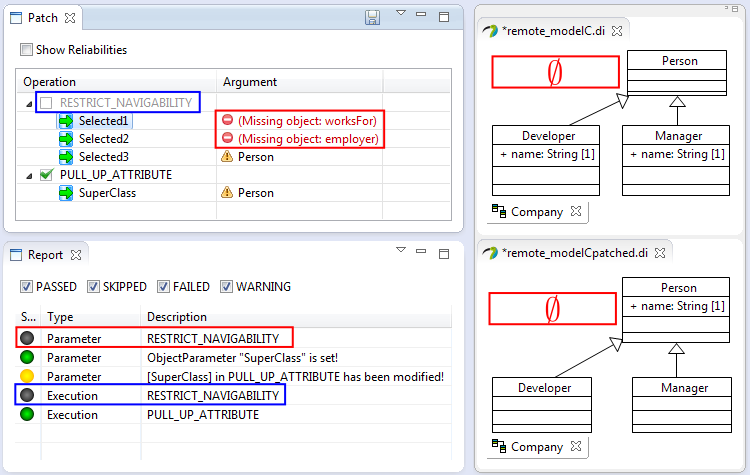
\includegraphics[scale=0.45]{images/patch_02_2}
  \end{center}
\end{frame}
\begin{frame}[noframenumbering]
  \frametitle{Controlled Merging (3)}
  \begin{center}
 % \includegraphics[scale=0.4]{images/applyPatchMerge} \\ 
 % \medskip
  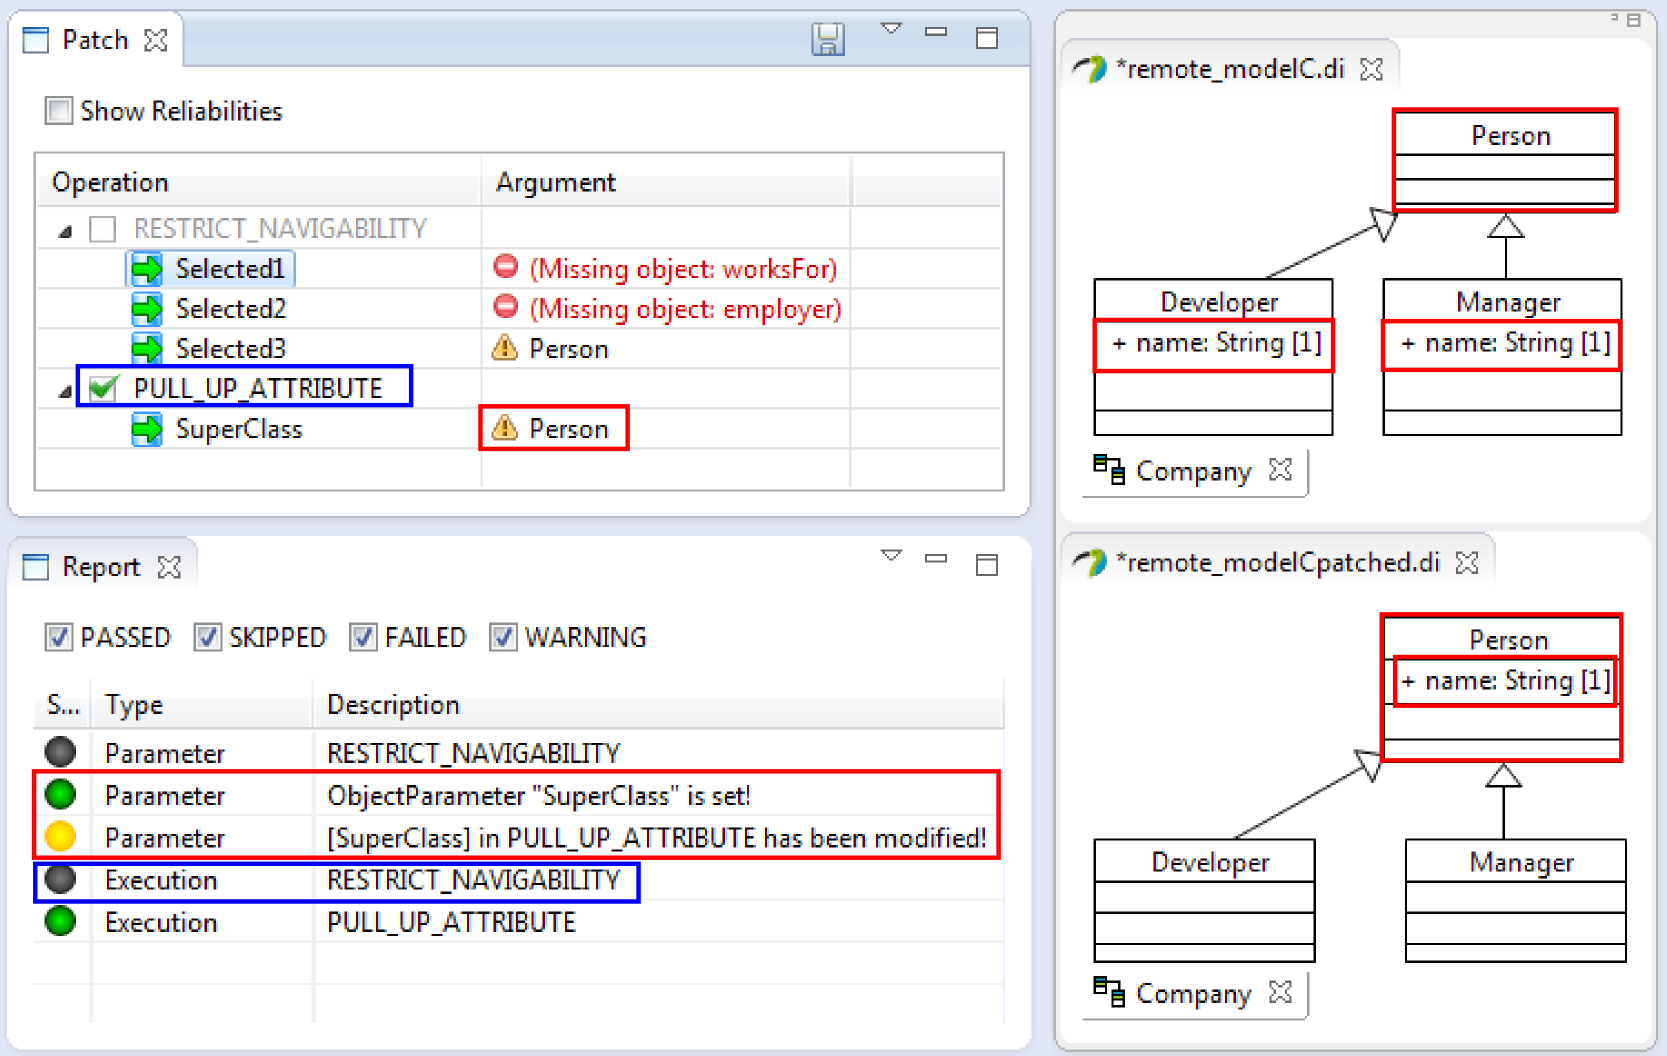
\includegraphics[scale=0.45]{images/patch_02_3}
  \end{center}
\end{frame}
\section{SiLift Approach}

\begin{frame}
  \frametitle{SiLift Pipeline (low level)}
  \begin{center}
  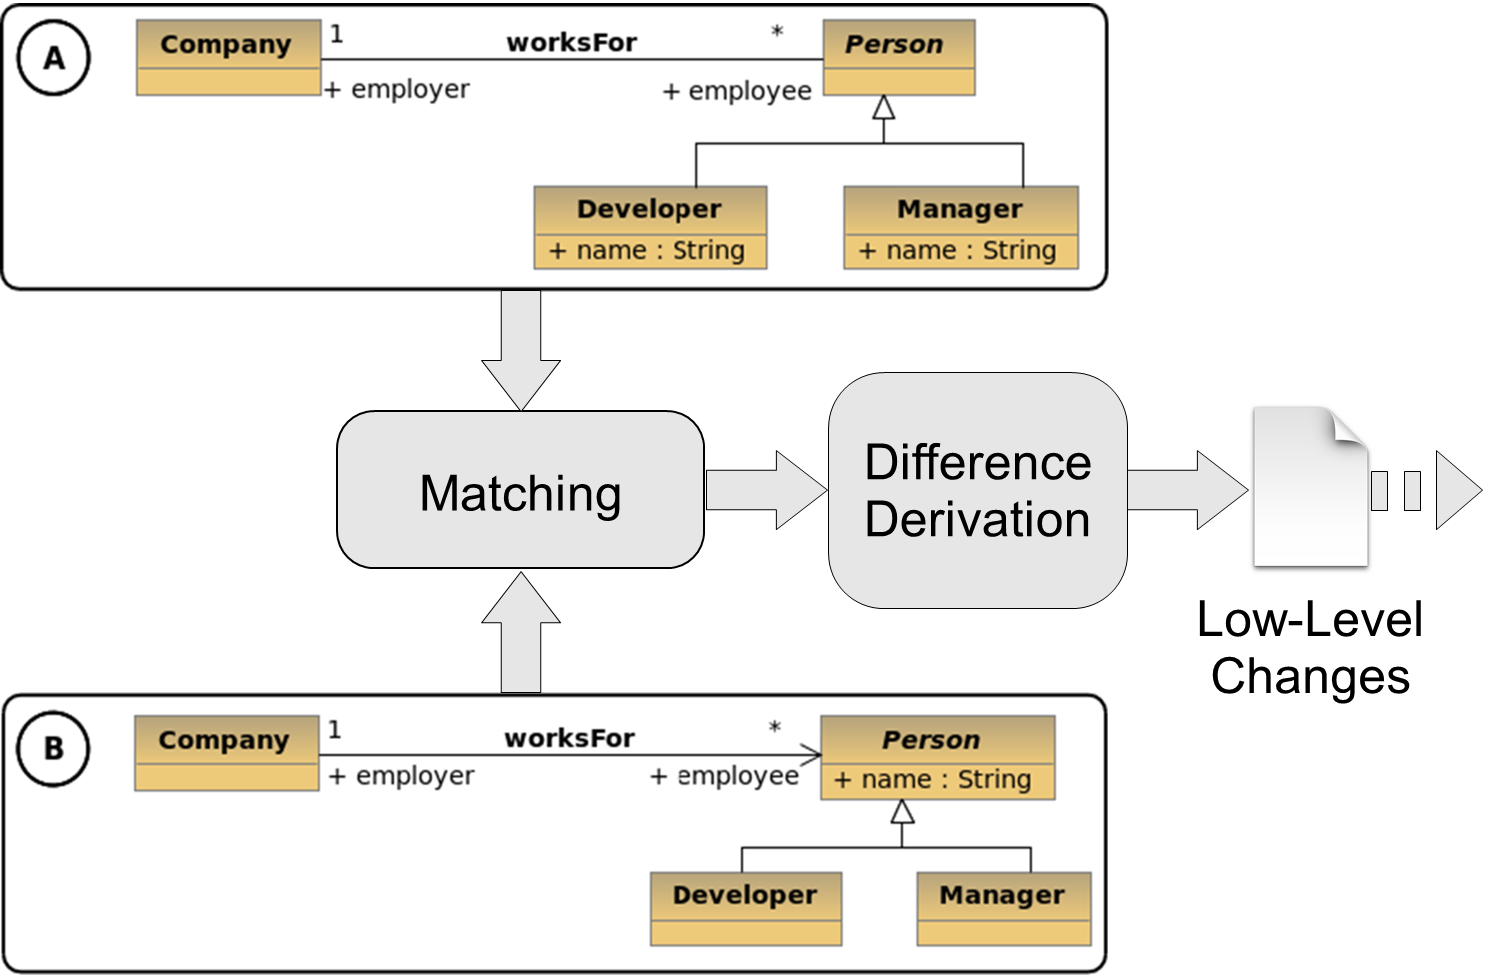
\includegraphics[scale=0.45]{images/pipeline_low-level}
  \end{center}
\end{frame}

\begin{frame}
  \frametitle{SiLift Pipeline (high level)}
  \begin{center}
  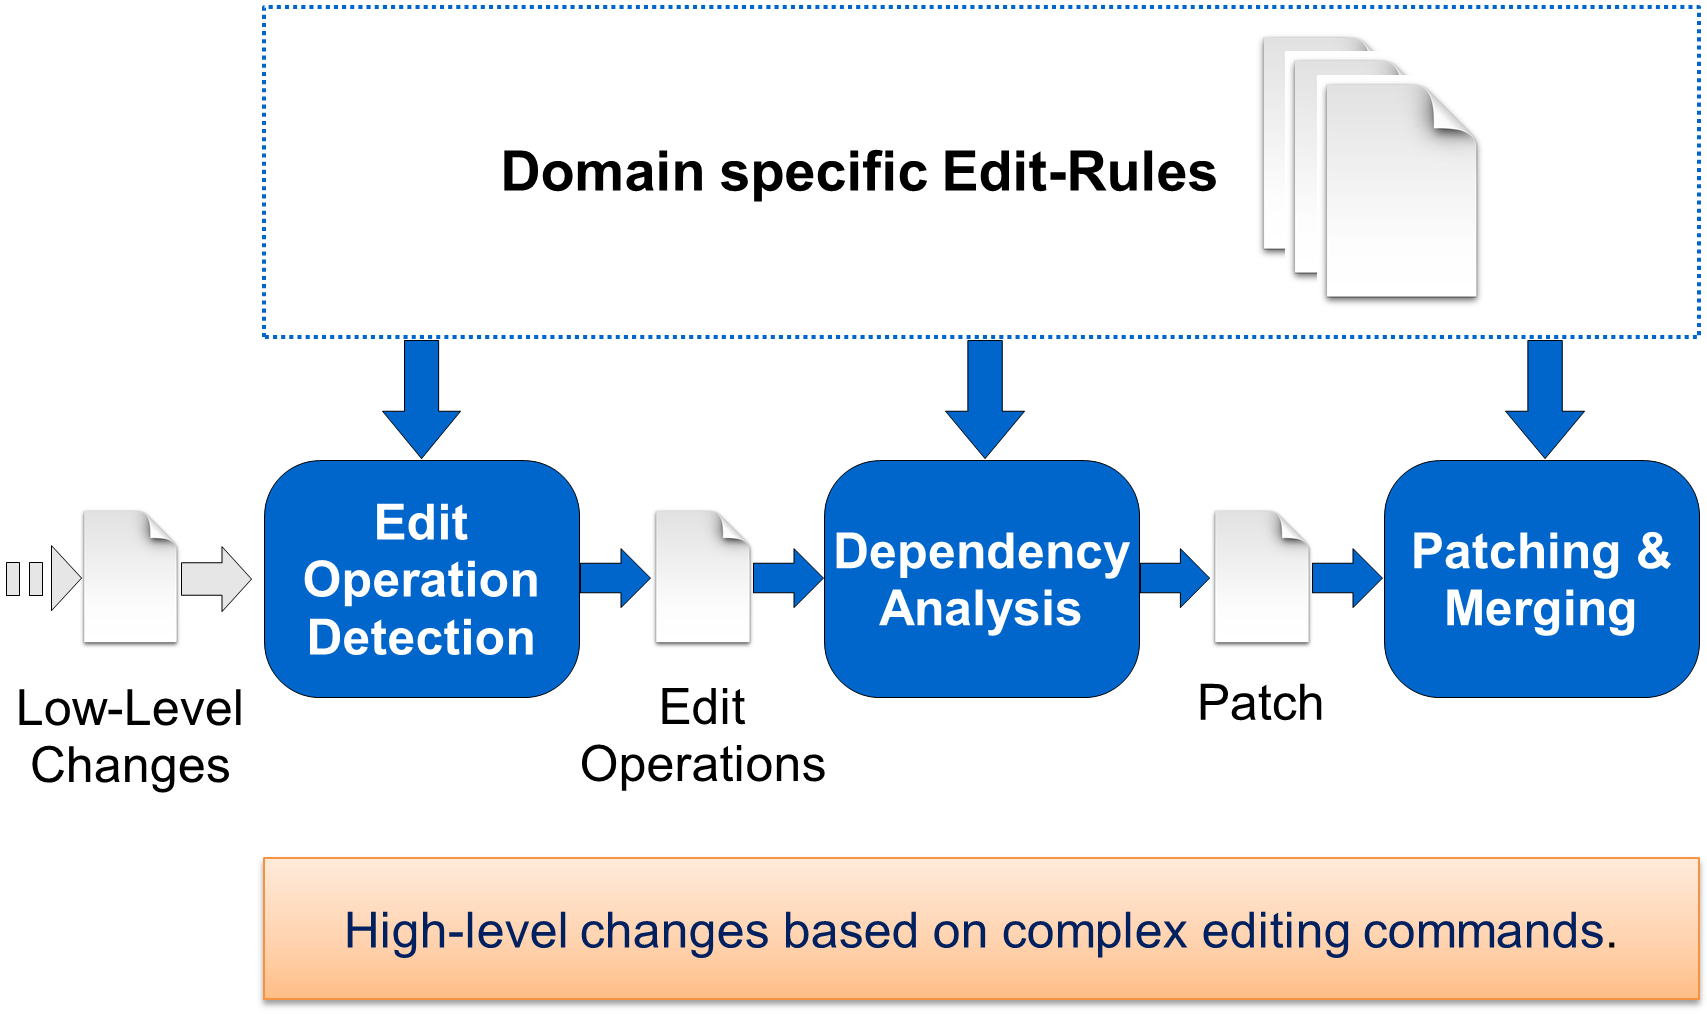
\includegraphics[scale=0.45]{images/pipeline_high-level}
  \end{center}
\end{frame}

\begin{frame}
  \frametitle{Theoretical Foundation}
  \begin{center}
  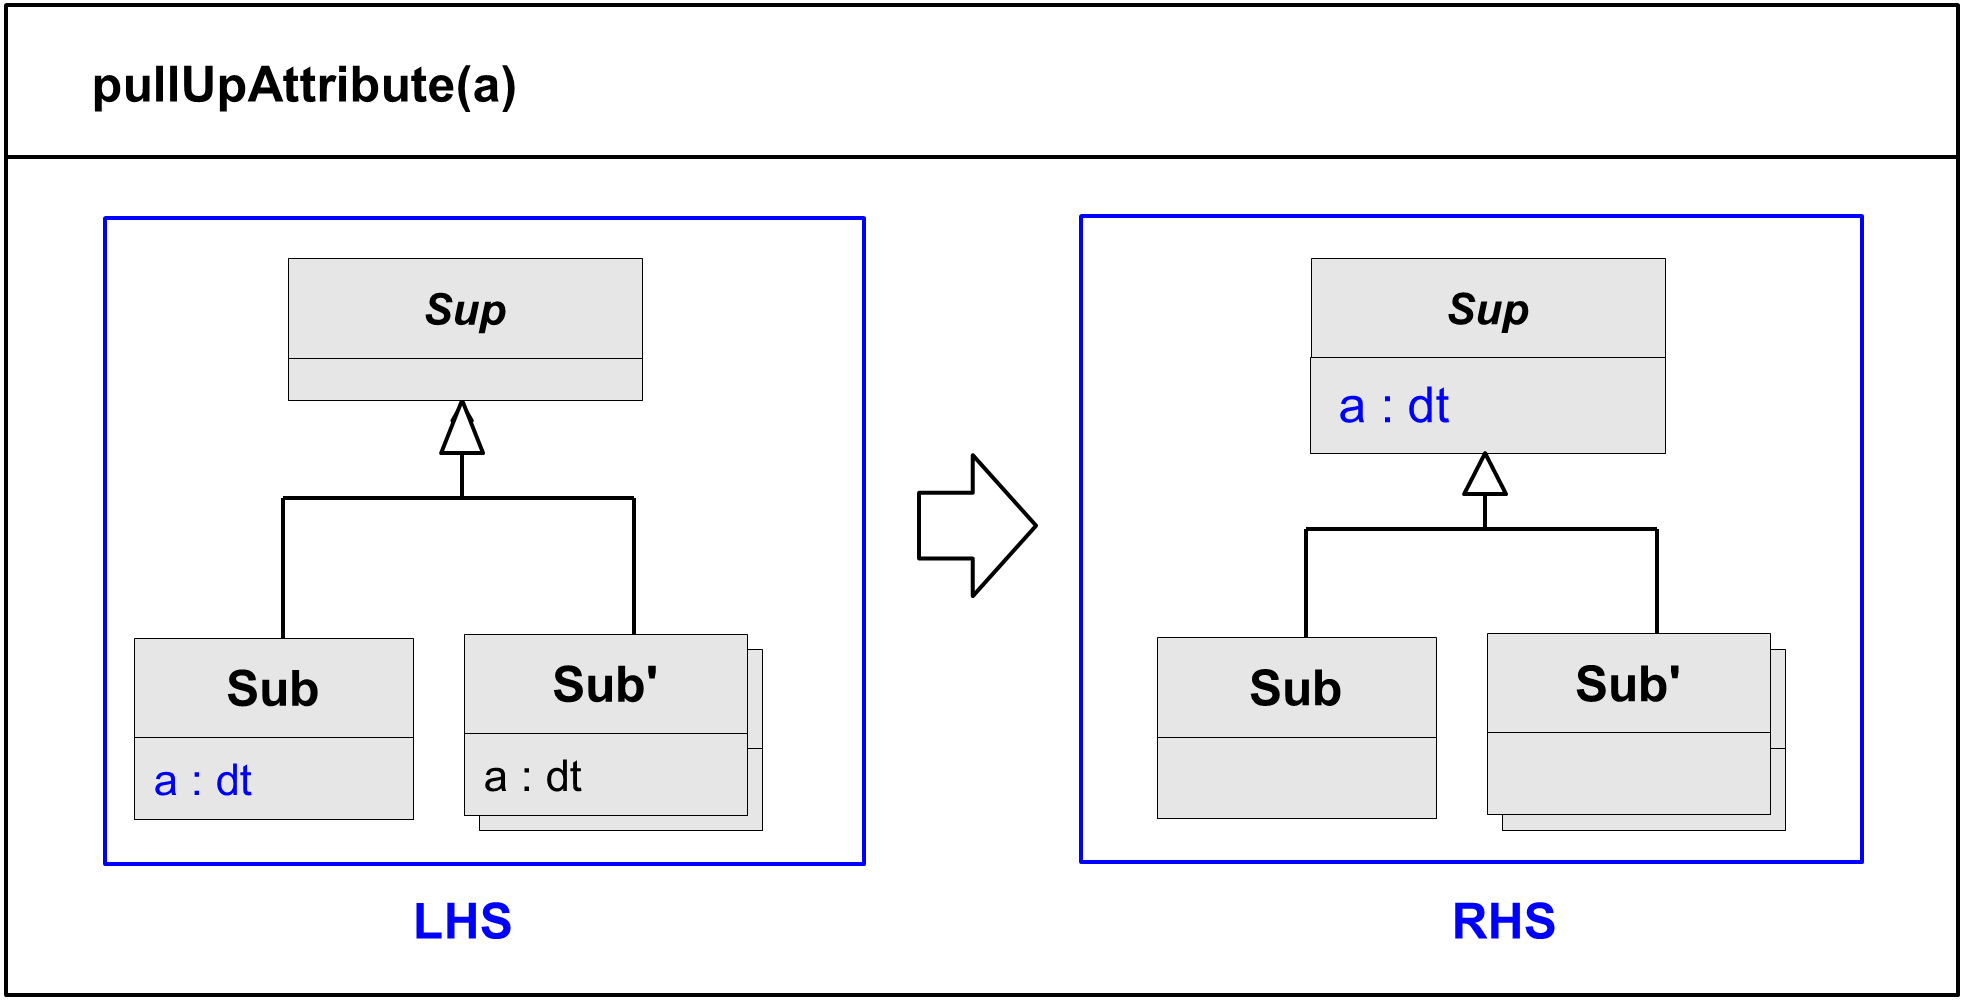
\includegraphics[scale=0.4]{images/graph_theory}
  \end{center}
\end{frame}

\begin{frame}
  \frametitle{Practical Usage}
  \begin{center}
  
\includegraphics[scale=2.0]{images/henshinLogo}\\
  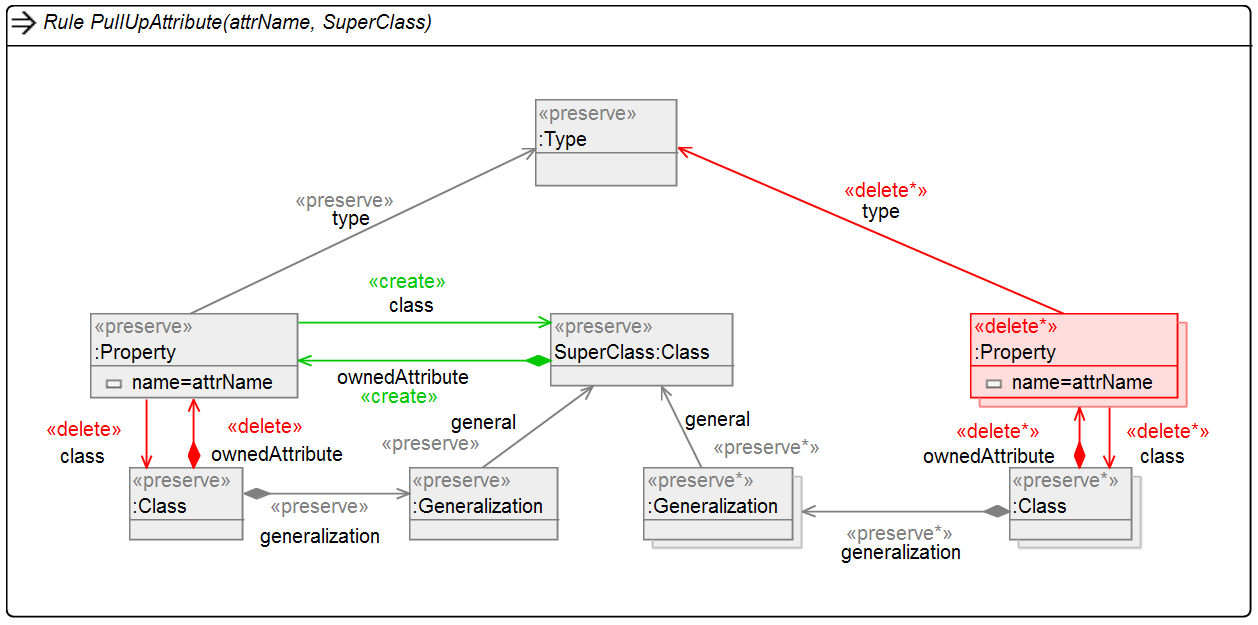
\includegraphics[scale=0.3]{images/pullUp_HR}
  \end{center}
\end{frame}
\section{Summary}
\begin{frame}
  \frametitle{Summary}  
  \begin{itemize}
    \item Edit Operations as \textbf{Building Blocks}
    \item Can be used in many scenarios:
    \begin{itemize}
      \item Differencing
      \item Patching
      \item \ldots
      \end{itemize}
      \item New Domain: New Pain
    \item Integrated Specifiation:
    \begin{itemize}
      \item Eclipse-based Technologies
      \item Editors/Projects
      \item Generated basic Edit Operation set
      \item Builder for derived artefacts
      \item Validation + Quickfixing
      \end{itemize}
  \end{itemize}
  \centering
 $\triangleright$ \textbf{New Domain - Less Pain}
  %\begin{block}{Achieved through}
  %\begin{itemize}
  %  \item Formal: Graph transformation concepts
  %  \item Practical: Henshin EMF
  %  \item Dependency and conflict detection
  %\end{itemize}
  %\end{block}
  \end{frame}
  \begin{frame}
 \frametitle{Contact/More information}
 \textbf{Download}
 \begin{itemize}
   \item Used Tools (including library meta model): \\
  \url{http://pi.informatik.uni-siegen.de/Projekte/SiLift/updatesite-edc14/}
  \item Example Instances + Edit Operations (as Projects): \\
    \url{http://pi.informatik.uni-siegen.de/Projekte/SiLift/downloads/edc14_example.zip}
 \end{itemize}
  \textbf{Web}
  \begin{itemize}
    \item \url{http://pi.informatik.uni-siegen.de/Projekte/SiLift}
  \end{itemize}
  \textbf{Email}
  \begin{itemize}
    \item \url{dreuling@informatik.uni-siegen.de} 
    \item \url{cpietsch@informatik.uni-siegen.de} 
  \end{itemize}
  \textbf{Personal}
  \begin{itemize}
    \item Now ;-)
  \end{itemize}
  \end{frame}


\end{document}
